%Packages used
\documentclass{article}
\usepackage[T1]{fontenc}
\usepackage[french]{babel}
\usepackage{titlesec}
\usepackage{blindtext}
\usepackage{graphicx}
\usepackage{float}
\usepackage{csquotes}
\usepackage[left=3cm,right=3cm,top=3cm,bottom=3cm]{geometry}
\usepackage{biblatex}
\usepackage{tabularx}
\usepackage{fancyhdr}
\usepackage{xcolor}
\usepackage{amsmath}

\addbibresource{Bibliography.bib}



% Set the page style to "fancy"...
\pagestyle{fancy}
%... then configure it.
\fancyhead{} % clear all header fields
\fancyhead[R]{{2230\_TubePitotDeporte-Rapport\_v1.0.0}}
\fancyfoot{} % clear all footer fields
\fancyfoot[C]{\thepage}


%Corps du document :
\begin{document} 

    
    
    \begin{titlepage}
    \begin{center}
        
        
        \null\vspace{2cm}
        {\huge Tube Pitot déporté} \\
        \textcolor{gray}{{Détection de l'angle d'incidence au décrochage d'un \\
        avion par mesure de la vitesse et des accélérations}}

        \vspace{0.5cm}
        Meven Ricchieri
        
        \textcolor{gray}{{2022 - 2023}}
        
    \end{center}

    
    \vspace{8cm}

    \begin{tabular} {l l l}

        Numéro de projet & : & 2230 \\\\\\
        
        
        
        Responsable & : & M. Juan José Moreno \\
        Mandataire & : & M. Vincent Seguin (pour AMPA)
        
    \end{tabular}
        
        
    \vspace{5cm}
        
    \begin{tabular} {cc}
        \parbox{0.3\textwidth}{
\includegraphics[width=4cm]{Images/ETML-ES.png}}
    \end{tabular}
    
    
\vspace{2cm}
\end{titlepage}
    \newpage
    \tableofcontents
    \newpage

    \section{Cahier des charges}
        Le but du projet consiste à développer un système permettant de détecter l’angle d’incidence et la vitesse au décrochage d’un avion. La fixation de ce système doit être flexible afin de pouvoir l’installer sur différents types d’avions. L’emplacement de fixation ne doit pas se trouver dans le flux d’air provenant de l’hélice afin d’éviter que la mesure de vitesse ne soit faussée. Il doit également être miniaturisé au maximum afin de produire le minimum de traînée possible et de ne pas dépasser un poids de 500g. Les données acquises par les capteurs doivent être transmises de la partie déportée à un appareil Android se trouvant dans le cockpit de l’avion au travers une communication sans fil. L’appareil Android doit traiter et afficher les données reçues, si possible graphiquement (optionnel). \\

\noindent Le cahier des charges complet se trouve en annexes.
\vspace{1 cm}


    \section{Pré-étude}
        \subsection{Contexte}
    Cette pré-étude consiste à mener des recherches qui conduirons à une décision de lancer ou non le projet. Cette décision va reposer sur les difficultés de réalisation électrique, mécanique et software. Elle va aussi permettre d'imaginer et de comparer les différentes manières de réaliser les tâches et ainsi choisir la meilleure. 
    \vspace{1 cm}
    
\subsection{Schéma de principe}
    \begin{figure}[h]
        \caption{Schéma de principe}
        \centering
        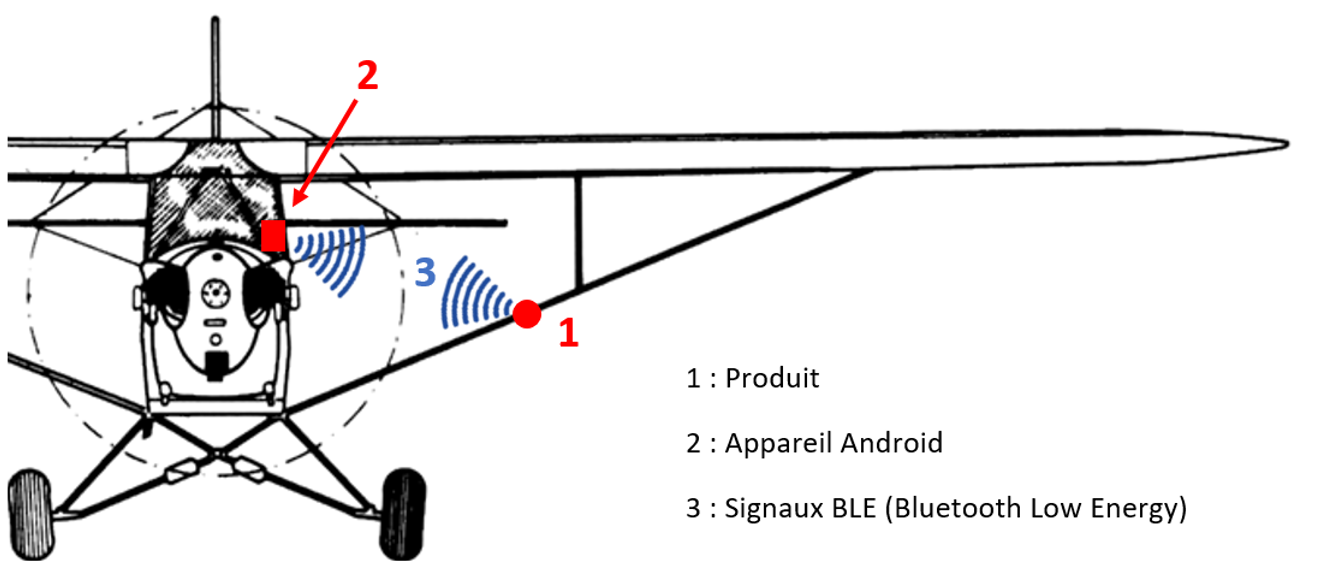
\includegraphics[width=15cm]{Images/piper-cub-j-3-3_modified2.png}
    \end{figure}
    \newpage
    
\subsection{Schéma bloc détaillé}
    \begin{figure}[h]
        \caption{Schéma bloc détaillé}
        \centering
        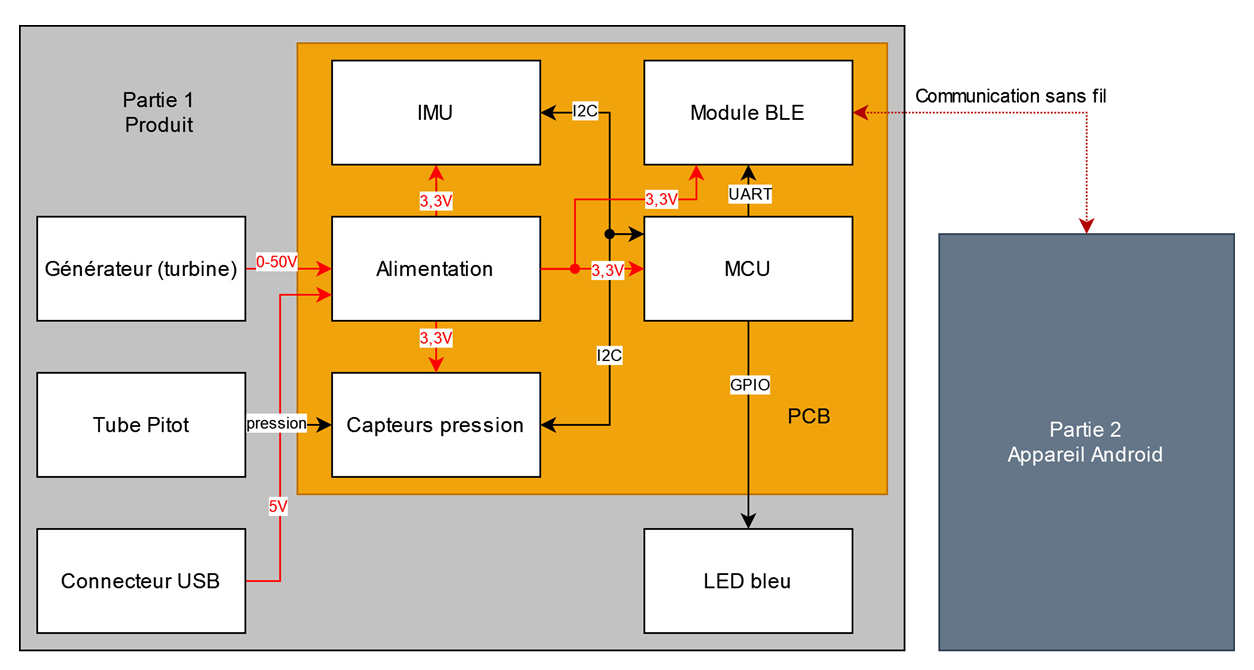
\includegraphics[width=15cm]{Images/SchemaBlocRapport_v1.0.1.drawio.png}
    \end{figure}
    \vspace{1 cm}
    
\subsection{Descriptions des blocs détaillées}
    
    \subsubsection{Bloc Générateur (turbine)}
        L’intérêt d’utiliser un générateur comme source d'énergie permet de simplifier l’utilisation du système, il n'y aura aucune maintenance à effectuer ou de batterie à charger. L'énergie cinétique de l'air en mouvement, par rapport à l'avion, vas être captée par les aubes de la turbine axée à un générateur, ce qui va produire une tension. Le système va se mettre en marche une fois que l'axe du générateur-turbine aura atteint une certaine vitesse de rotation. Plus la vitesse sera grande, plus la tension générée sera élevée. Un simple moteur DC, va permettre de transformer cette énergie mécanique en énergie électrique. Il est possible d'utiliser d'autres technologies comme les moteurs brushless, qui ont un rendement bien meilleur, mais cela complexifie le circuit et augmente le prix. Dans ce projet, le rendement n'est pas primordial car le système ne consommera que très peu d'énergie.
        \begin{equation}
            U_{t}(V) = \frac{n}{k_{n}}-R_{mot}*I_{L} \text{ \cite{noauthor_maxon_nodate}}
        \end{equation}
        où:
        
        \begin{tabular}{l l l}
            $U_{t}$ & = & Tension aux bornes du moteur DC (V) \\
            $k_{n}$ & = & Constante de vitesse du moteur DC (rpm/V) \\
            $R_{mot}$ & = & Résistance aux bornes du moteur DC ($\Omega$) \\
            $n$ & = & Vitesse moteur DC (rpm) \\
            $I_{L}$ & = & Courant de charge (I) \\
        \end{tabular}
        \vspace{0.5 cm}
        \noindent Puisque la valeur de la tension générée est dépendante de la vitesse air de l'avion, celle-ci ne sera jamais stable. Il faudra donc la transformer et la réguler avant de la transmettre aux composants électroniques, ce à quoi le bloc "Alimentation" sera destiné.
        
        
        \newpage
        \noindent N'ayant pas de grandes connaissances dans le dimensionnement et le design de générateur-turbines, des recherches plus poussées seront nécessaires afin de rendre le système performant. Pour me faire une première idée, j'ai dessiné et imprimé une première turbine composée de 13 aubes puis j'ai effectué quelques tests. A l'aide d'un moteur DC, j'ai réussi à générer une tension d'environ 3V à une vitesse de 80km/h.

        \begin{figure}[h]
            \caption{Turbine de test N°1}
            \centering
            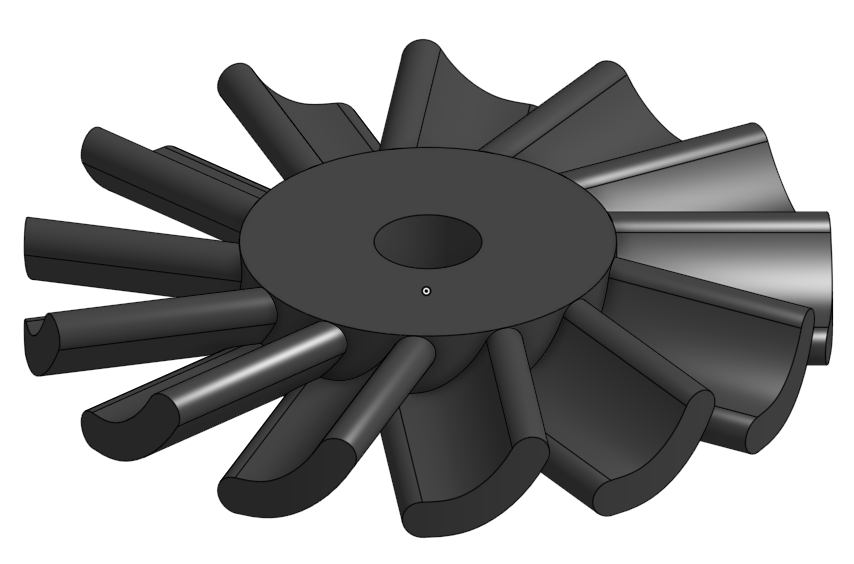
\includegraphics[width=7cm]{Images/TurbineTest.png}
        \end{figure}
        \vspace{1 cm}
    
    \subsubsection{Bloc Capteur de pression}
        Le système sera équipé d'un capteur de pression différentielle qui permettra de mesurer la différence entre la pression statique et la pression totale.
        \emph{"La pression statique, dans un fluide en mouvement, est la pression que mesure un capteur qui se déplace à la même vitesse que le fluide"} \cite{noauthor_pression_2020}.
        \emph{"La pression totale dans un fluide (eau, air, etc.) est la somme de la pression statique, de la pression dynamique, et de la densité volumique d'énergie potentielle de gravité"} \cite{noauthor_pression_2022}. Grâce aux valeurs ainsi mesurées, il sera possible de calculer la vélocité du fluide, ce qui correspondra à la vitesse air de l'avion. Pour des vitesses inférieures à Mach 0.3 (200 nœuds), l'effet de compressibilité du fluide peut être négligé \cite{noauthor_tube_2022}.
        \begin{equation}
            v(m/s) = \sqrt{\frac{2*(p_{t}-p_{s})}{\rho}} \text{ \cite{noauthor_tube_2022}}
        \end{equation}
        où:
        
        \begin{tabular}{l l l}
            $v$ & = & Vélocité du fluide (m/s) \\
            $p_{t}$ & = & Pression totale (Pa) \\
            $p_{s}$ & = & Pression statique (Pa) \\
            $\rho$ & = & Masse volumique du fluide ($kg/m^3$) \\
        \end{tabular}
        \vspace{1cm}
    
    
    \subsubsection{Bloc Tube Pitot}
        Comme expliqué au point précédent, la vitesse se calcule grâce à la pression statique et totale, pour que le capteur différentielle ait accès à ces deux pressions, il faut ajouter deux entrées d'air. Ces entrées doivent être placées correctement car dans le cas contraire, la vitesse calculée ne sera pas correcte. L'entrée de la pression statique doit être perpendiculaire à l'écoulement local du fluide (non perturbé) alors que celle de la pression totale doit être parallèle à ce flux. Il existe 3 tubes différents, le premier, appelé tube Pitot simple, est simplement un tube perforé en son centre faisant office d'entrée d'air pour la pression totale. Le second, appelé sonde statique, est perforé latéralement permettant l'entrée d'air pour la pression statique. Le troisième est une combinaison des deux premiers, il dispose d'une entrée pour la pression totale et d'une autre pour la pression statique. L'idéal serait d'utiliser ce dernier car il simplifierait l'implémentation mécanique du système. Les deux sorties du tube seraient reliées au capteur de pression différentielle par des tuyaux. Dans le cas ou un tube Pitot simple serait utilisé, il serait nécessaire de perforer le boîtier du produit afin d'avoir accès à la pression statique.
        La décision du type de tube sera effectué lors du design mécanique car il n'influence aucunement la conception électronique.
        \begin{figure}[h]
            \caption{Types de tubes Pitot}
            \centering
            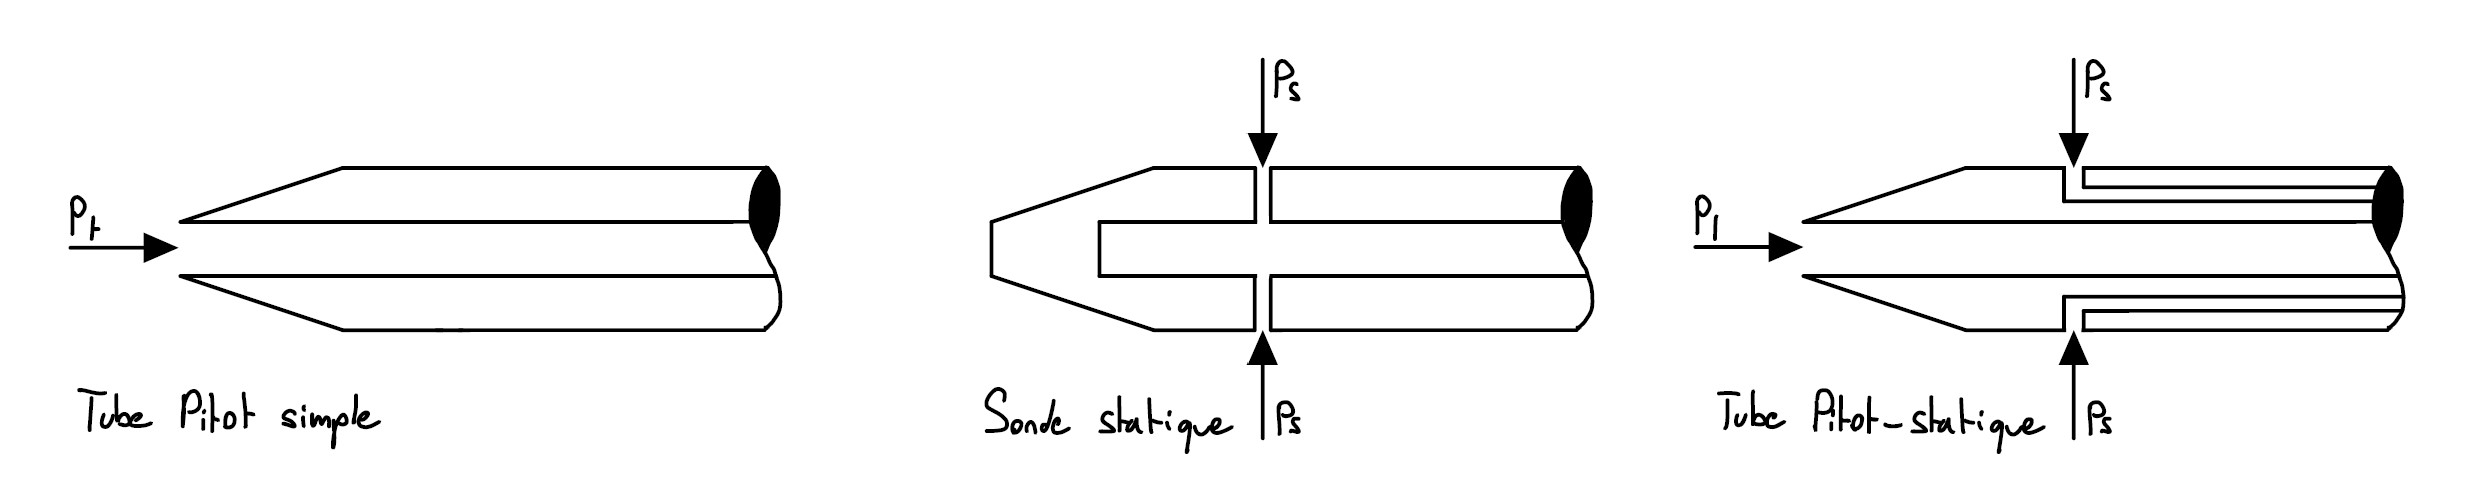
\includegraphics[width=15cm]{Images/TubesPitot.jpg}
        \end{figure}

    \subsubsection{Bloc IMU}
        La centrale inertielle comportera 6 capteurs, 3 gyromètres et 3 accéléromètres. \emph{"Les gyromètres mesurent les trois composantes du vecteur vitesse angulaire (vitesses de variation des angles de roulis, de tangage et de lacet. Les accéléromètres mesurent les trois composantes du vecteur force spécifique. La force spécifique est la somme des forces extérieures autres que gravitationnelles divisée par la masse"} \cite{noauthor_centrale_2022}.
        C’est grâce à ses capteurs qu’il sera possible de détecter le moment où l'avion commence à décrocher. La plupart de ces IMUs ont également un capteur de température intégré, la mesure de cette grandeur peut être intéressante puisqu'elle a une influence sur la valeur de la pression.
        \begin{figure}[ht]
            \caption{Données mesurés par l'IMU}
            \centering
            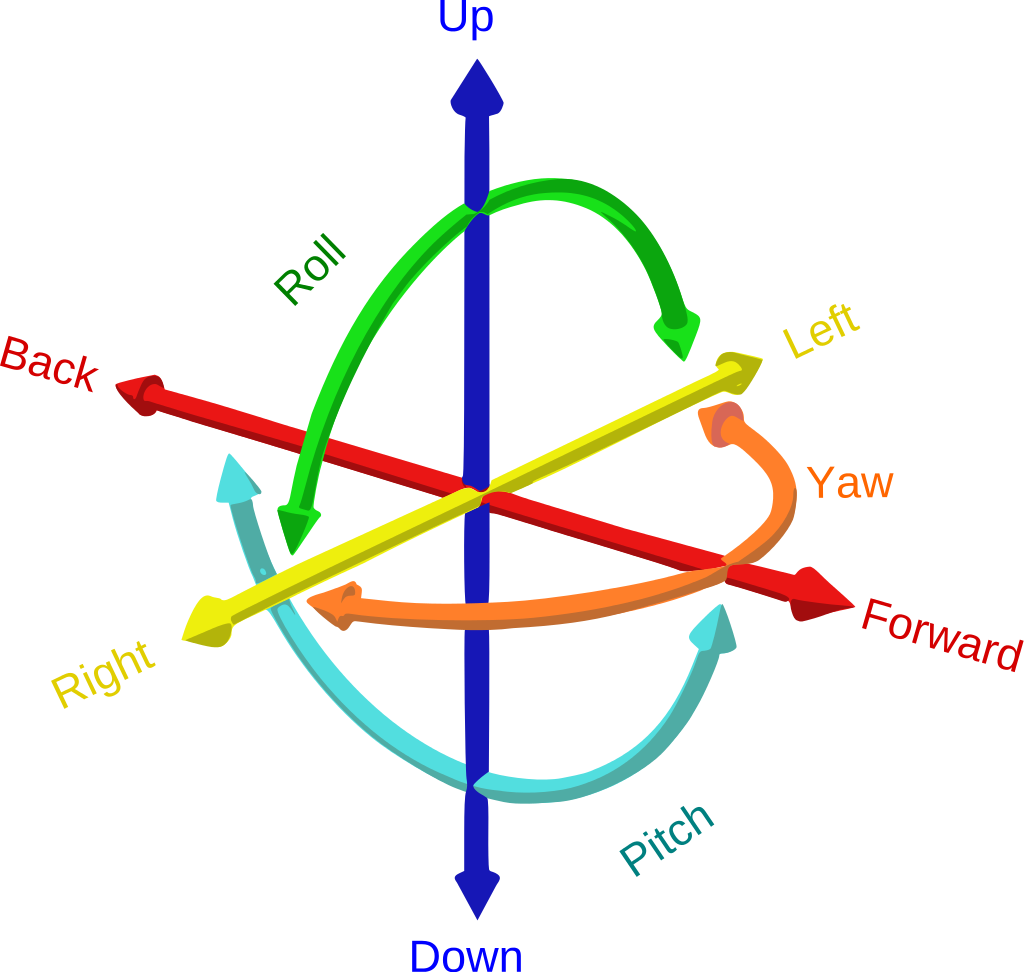
\includegraphics[width=5cm]{Images/6axes.png}
        \end{figure}
        \vspace{1cm}
    
    \subsubsection{Bloc Connecteur USB}
        Étant donné que le système n'aura pas de source d'énergie interne, un connecteur USB-C sera implémenté afin de pouvoir tester la communication ainsi que les capteurs, en amont du vol. Il permettra également d'alimenter le système lors de son installation sur l'avion, car il devra être positionné correctement à l'horizontale pour que les mesures soient fiables.\newpage
        
    \subsubsection{Bloc Module BLE}
        Le transfert de données entre le produit et l'appareil Android, se fera au travers d'une communication sans fil Bluetooth Low Energy (BLE). Cette variante de Bluetooth permet de réduire significativement sa consommation par rapport au mode normal. Il sera tout de même possible qu'un module permettant de choisir le mode de fonctionnement soit implémenté. Les données transmises du produit à l'appareil Android seront principalement les valeurs lues par les capteurs alors que celle provenant de l'appareil seront plutôt des commandes ou réglages.\vspace{1cm}
    
    \subsubsection{Bloc LED bleue}
        Comme énoncé dans le CDC, la LED bleue va permettre d'indiquer l'état du système. La LED éteinte va signifier que le système n'est pas alimenté. Un clignotement toute les 2 secondes correspondra au système alimenté mais non appairé à un périphérique Bluetooth et finalement, 2 clignotements toute les 2 secondes correspondra à l'état fonctionnel, appairé et transmettant les données. La LED devra être visible de jour donc son emplacement et son intensité lumineuse devront être correctement défini.\vspace{1cm}

    \subsubsection{Bloc MCU}
        Le microcontrôleur sera obligatoirement un modèle 32Bit du fabriquant Microchip. Il va faire le lien entre tous les périphériques implémentés, c'est à dire les composants d'entrées, IMU et capteur de pression et ceux de sortie, module BLE et LED.
        Selon les recherches effectués précédemment, le microcontrôleur devra au minimum contenir, \\
        \begin{itemize}
            \item Un module UART pour la communication avec le module Bluetooth
            \item Un module I2C pour la communication avec l'IMU
            \item Une PIN GPIO pour le contrôle de la LED
        \end{itemize}
        \vspace{1cm}

\subsubsection{Bloc Alimentation}
    Puisque la grande majorité des composants nécessaires, tel que le PIC ou les capteurs, fonctionnent avec une tensions de 3.3V, il faudra donc que la sortie de ce bloc soit proche de cette valeur. Le générateur va produire une tension bien supérieur à 3.3V, donc la meilleure option est d'utiliser un convertisseur Buck afin de l'abaisser. Il permettra d'avoir un bien meilleur rendement qu'un régulateur linéaire et donc limiter la consommation.
    \begin{table}[h!]
        \centering
        \begin{tabular}{| l || r | r |}
            \hline
            Composant & min & max \\
            \hline
            Module BLE (consommation non continue)  & 5mA & 10mA \\
            Microcontrôleur & 5mA & 10mA\\
            Capteur pression différentielle & 3mA & 4mA \\
            LED (consommation non continue) & 10mA & 20mA \\
            Centrale inertielle & 1mA & 3mA \\
            \hline
            Total & 24mA & 47mA\\
            \hline
        \end{tabular}
    \end{table}
    
    La consommation totale devrait se situer entre 24mA et 47mA\newpage

        
        
    \subsubsection{Bloc Appareil Android}
        Toutes les données obtenues au travers de la communication sans fil seront traitées et affichées sur l'écran de l'appareil. Ces données seront affichées sous forme numérique et dans l'idéal, sous forme graphiques, mais cela reste optionnel. L'application permettra d'envoyer certaines commandes au produit en appuyant sur les différents boutons qui seront affichés. Il sera aussi possible d'ajouter une valeur d'offset aux mesures pour compenser une éventuelle erreur. 
        \vspace{1cm}
        
\subsection{Design mécanique}
    Comme expliqué dans le cahier des charges, l'idée est d'adapter tout le système pour qu'il puisse se trouver dans un cylindre à l'arrière du tube Pitot. Le boîtier et les autres parties mécaniques seront imprimé en une matière plastique selon la disponibilité de matériaux de l'école. L'idéal serait d'utiliser de l'acrylonitrile butadiène styrène (ABS) car ses caractéristiques mécaniques sont bien supérieures à l'acide polylactique (PLA). La grosse difficulté va être de miniaturiser le design du PCB afin de rendre la section du tube la plus mince possible. Le système de fixation sera réalisé grâce à une boule style RAM-Mounts vissé au boîtier. 
    
    \begin{figure}[h]
        \caption{Premier croquis du design mécanique}
        \centering
        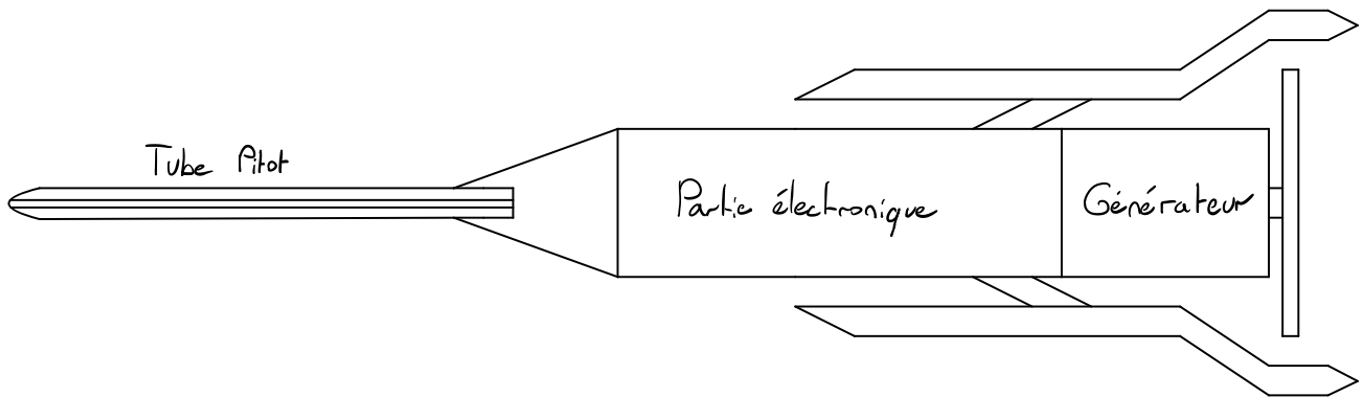
\includegraphics[width=15cm]{Images/CroquisMecanique.png}
    \end{figure}
    \newpage
    
\subsection{Estimation du prix}
    L'estimation du prix est actuellement difficile car certains choix doivent encore êtres pris et la disponibilité des composants peut avoir une influence, j'ai donc mis un plage de prix.

    \begin{table}[h!]
    \centering
    \begin{tabular}{| l || r | r |}
        \hline
            Composant & min & max \\
            \hline
            Générateur (moteur DC) & 5.- & 50.- \\
            Turbine (ABS) & 0.5.- & 1.- \\
            Capteur pression différentielle & 30.- & 70.- \\
            Tube Pitot & 0.- & 30.- \\
            Centrale inertielle & 5.- & 12.- \\
            Connecteur USB-C & 1.- & 3.- \\
            Module Bluetooth & 5.- & 15.- \\
            LED & 0.5.- & 3.- \\
            MCU & 1.- & 3.- \\
            Convertisseur Buck & 3.- & 8.- \\
            Boîtier (ABS) & 1.- & 2.- \\
            Boule RAM-Mounts & 15.- & 25.- \\
            PCB & 50.- & 75.- \\
            \hline
            Total & 126.- & 396.-\\
        \hline
     \end{tabular} 
     \end{table}
    Le prix devrait se situer entre 126.- et 396.-
    \vspace{1cm}

\subsection{Faisabilité du projet}
    D'après les informations trouvées, le projet est totalement réalisable. Il y aura sans doutes quelques difficultés au niveau du dimensionnement de la partie turbine-générateur.
    \newpage
    \section{Design électronique}
        \input{Documents/DesignElectronique.tex}
    %\section{Conclusion}
        %\input{Documents/Conclusion.tex}
    \section{Annexes}
        \begin{tabular}{l l}
            - & Référence \\
            - & Cahier des charges \\
        \end{tabular}

    \newpage
    \printbibliography
    \clearpage


\end{document}


